\documentclass[11pt]{article}

\usepackage[margin=1in]{geometry}
\usepackage{amsmath}
\usepackage{amssymb}
\usepackage{mathtools}
\usepackage{booktabs}
\usepackage{longtable}
\usepackage{graphicx}
\usepackage{microtype}
\usepackage{enumitem}
\usepackage{hyperref}
\usepackage{natbib}
\usepackage{caption}
\usepackage{subcaption}
\usepackage[T1]{fontenc}
\usepackage{lmodern}
\usepackage{xcolor}
\usepackage{flafter}

\hypersetup{
    colorlinks=true,
    linkcolor=black,
    citecolor=black,
    urlcolor=blue
}

\setlist[itemize]{leftmargin=1.5em}
\setlist[enumerate]{leftmargin=1.7em}
\setlength{\parskip}{0.45em}
\setlength{\parindent}{0pt}

\title{\textbf{Scaling SOAP for Tensor-Parallel Training on Frontier}\\
\large 2026 Oak Ridge National Laboratory Internship Report}
\author{Ritvik Prabhu\\
Mentors: Aditya Kashi and Sajal Dash}
\date{August 2026}

\begin{document}

\maketitle

\section*{Executive Summary}

This internship investigated whether SOAP, a matrix-based optimizer, can be made practical for tensor-parallel training on Frontier. SOAP uses Shampoo-style matrix statistics and applies Adam in a basis derived from the preconditioners \citep{vyas2024soap}. I built a distributed implementation for row- and column-sharded matrices that keeps the main optimizer state distributed across GPU ranks and uses ELPA and SLATE for the required eigensolver, QR, and matrix operations.

The distributed preconditioner, rotation, and Adam components matched dense references closely, generally near the $10^{-7}$ relative-error level in the component tests. Larger differences appeared in the complete SOAP update, especially as matrix size increased. Further experiments showed that much of this divergence was associated with differences in the eigenbasis rather than the distributed matrix operations themselves. This is important because SOAP stores Adam state in the rotated coordinates, making the optimizer sensitive to otherwise valid changes in the basis.

The implementation also showed useful strong scaling on Frontier. For a $16{,}384\times16{,}384$ matrix, the average SOAP step decreased from approximately 81.9 seconds on one GPU rank to 25.0 seconds on eight ranks, giving a $3.27\times$ speedup. The next steps are to optimize the current workflow, investigate whether the two-dimensional block-cyclic layout can be avoided, study basis stability and rank-deficient preconditioners, and overlap SOAP work with backpropagation.


\section{Internship Scope and Research Question}

The internship began with a broader interest in curvature-aware optimization for large machine-learning workloads. I wanted to understand whether an optimizer with richer matrix structure than AdamW could remain practical when the model itself is distributed across GPUs.

This is partly an algorithmic question and partly a systems question. An optimizer may reduce the number of training steps while adding enough per-step cost to erase that advantage. At scale, the relevant costs include optimizer state, communication, matrix factorizations, and synchronization between ranks.

I eventually narrowed the project to SOAP and the following question:

\begin{quote}
Can SOAP operate directly over tensor-parallel Transformer shards while keeping its large matrix state and matrix operations distributed?
\end{quote}

The implementation was designed around three requirements. It needed to support both row- and column-sharded matrices, preserve the main SOAP update, and scale across multiple GPU ranks without reconstructing the complete gradient on a single device.

I evaluated the resulting implementation on Frontier using 1, 2, 4, and 8 GPU ranks.

\section{Background and Motivation}

\subsection{From Adam to matrix preconditioning}

Adam maintains exponential moving averages of the gradient and squared gradient and uses them to scale each parameter independently \citep{kingma2014adam}. AdamW separates weight decay from the adaptive update \citep{loshchilov2017adamw}. Their elementwise structure is useful in distributed training because the optimizer state can follow the same partitioning used for parameters and gradients.

For a matrix parameter, however, an elementwise optimizer does not explicitly model relationships between different rows or columns. Matrix-based optimizers introduce this structure through larger statistics computed from the gradient.

Shampoo is one example. For a matrix gradient $G$, it maintains statistics based on $GG^\top$ and $G^\top G$ \citep{gupta2018shampoo}. These matrices capture relationships along the two dimensions of the parameter. The added structure comes with larger state and more expensive linear algebra.

I use the terms \emph{preconditioned} and \emph{curvature-aware} in this report. SOAP does not form or invert the exact Hessian, so describing it as a full second-order method would be misleading.

\subsection{SOAP}

SOAP combines Shampoo-style matrix statistics with Adam \citep{vyas2024soap}. For a gradient
$G_t \in \mathbb{R}^{m \times n}$, its left and right preconditioners are updated as

\begin{align}
L_t &= \beta L_{t-1} + (1-\beta)G_tG_t^\top, \\
R_t &= \beta R_{t-1} + (1-\beta)G_t^\top G_t.
\end{align}

Let $Q_L$ and $Q_R$ denote orthogonal bases associated with $L_t$ and $R_t$. SOAP projects the gradient into those coordinates:

\begin{equation}
Z_t = Q_L^\top G_t Q_R.
\end{equation}

Adam then operates on $Z_t$. If $C_t$ is the resulting update in the projected coordinates, SOAP maps it back to the parameter coordinates using

\begin{equation}
U_t = Q_L C_t Q_R^\top.
\end{equation}

The appeal of SOAP is the tradeoff between a more expensive optimizer step and potentially faster convergence. The SOAP paper reports improvements in both training-step efficiency and wall-clock time relative to AdamW for the language-model workloads it evaluates \citep{vyas2024soap}.

For this project, SOAP was also useful because its computational stages are clearly identifiable. Preconditioner construction, basis calculation, projection, Adam, and the backward rotation can all be implemented and tested separately.

\subsection{The tensor-parallel problem}

Tensor parallelism splits a single model matrix across several GPUs. Consider a column-sharded gradient

\begin{equation}
G = [G_0 \; G_1 \; \cdots \; G_{p-1}],
\end{equation}

where rank $r$ stores $G_r \in \mathbb{R}^{m \times n_r}$.

The left Gram matrix is relatively convenient:

\begin{equation}
GG^\top =
\sum_{r=0}^{p-1} G_rG_r^\top.
\end{equation}

Each rank can compute a local contribution before the partial results are combined.

The right Gram matrix contains cross-rank terms:

\begin{equation}
G^\top G =
\begin{bmatrix}
G_0^\top G_0 & G_0^\top G_1 & \cdots \\
G_1^\top G_0 & G_1^\top G_1 & \cdots \\
\vdots & \vdots & \ddots
\end{bmatrix}.
\end{equation}

Its off-diagonal blocks depend on columns held by different ranks. The row-sharded case has the same issue on the opposite side.

The basis rotations create another distributed matrix problem. Both
$Q_L^\top GQ_R$ and $Q_L C Q_R^\top$ couple information across the matrix dimensions. Basis initialization and refresh also require eigensolver or QR operations on matrices that are larger than a single tensor-parallel shard.

This turned the project into a distributed numerical linear algebra problem inside the optimizer.

\section{Prior Work and Research Gap}

Several existing systems address pieces of this problem.

Distributed Shampoo scales Shampoo-style preconditioning across distributed training by partitioning preconditioner state and computation \citep{shi2023distributedshampoo}. It demonstrates that matrix-based optimizers can be distributed successfully, while also showing that blocking and communication strategy have a large effect on cost.

NVIDIA has explored layer-wise distributed optimizer strategies for emerging matrix-based optimizers \citep{nvidia2026layerwise,nvidia2026emerging}. In that design, complete layers can be assigned to particular ranks so that the optimizer operates on an intact tensor.

Canzona considers matrix-based optimizers under both data-parallel and tensor-parallel fragmentation and uses asynchronous scheduling and load balancing to distribute optimizer work \citep{wang2026canzona}. This is closer to the setting I was studying.

These systems changed how I framed the internship. The useful research question was narrower than ``how to distribute SOAP.'' I focused on a SOAP-specific path in which the matrix operations themselves are executed over tensor-parallel shards. Preconditioner construction, basis work, projection, optimizer state, and the final rotation all remain distributed throughout the update.

The public SOAP implementation provides an important reference point. It exposes a configurable maximum preconditioner dimension, with a default value of 10,000 in the public code \citep{soapgithub}. I treat this as an implementation choice rather than a mathematical limitation of SOAP. The relevant distinction for this project is that the reference path assumes the matrix used by the optimizer can be materialized locally.

\section{Design and Implementation}

\subsection{Distributed data model}

The optimizer begins with the layout already used by tensor parallelism. A column-sharded parameter gives each rank a matrix
$G_r \in \mathbb{R}^{m \times n_r}$, while a row-sharded parameter gives each rank
$G_r \in \mathbb{R}^{m_r \times n}$.

SOAP introduces several matrices with different shapes. The left preconditioner and basis are $m \times m$. The right preconditioner and basis are $n \times n$. The projected gradient and Adam state span the original $m \times n$ parameter space in the rotated coordinates.

I distribute these matrices over a two-dimensional process grid using a block-cyclic layout. This layout is convenient for the dense distributed operations used later in the SOAP step.

The implementation therefore moves between two representations. The tensor-parallel layout is used by the model, while the block-cyclic layout is used by the distributed linear algebra routines. The gradient is redistributed before the matrix operations begin, and the completed SOAP update is redistributed back to the original tensor-parallel partition.

Block size is configurable. Smaller blocks tend to improve load balance, although they create more tiles and additional communication overhead. Larger blocks reduce bookkeeping and can work well when the matrices are large enough to provide sufficient work per rank. I left this as a tuning parameter because the best choice depends on both matrix size and process-grid shape.

\subsection{Distributed preconditioner construction}

For every matrix gradient, SOAP updates

\begin{align}
L_t &= \beta L_{t-1} + (1-\beta)G_tG_t^\top, \\
R_t &= \beta R_{t-1} + (1-\beta)G_t^\top G_t.
\end{align}

The communication pattern depends on how the model tensor is sharded.

For a column-sharded gradient, each rank can form its local contribution to
$GG^\top$. Those partial matrices are reduced into the owners of the corresponding block-cyclic tiles.

Constructing $G^\top G$ requires cross-rank products. I exchange gradient panels between ranks and form the required off-diagonal blocks directly. Each result is accumulated by the rank that owns that block of the distributed right preconditioner.

For a row-sharded gradient, these roles are reversed. The right Gram matrix can be formed from local contributions, while the left Gram matrix requires products between row panels held on different ranks.

The preconditioners are symmetric positive semidefinite. Where supported by the downstream operation, the implementation works with one triangular half of the matrix. This avoids constructing and communicating both copies of each symmetric tile.

I implemented and tested the four combinations separately: left and right preconditioners for both row- and column-sharded inputs. Keeping these tests independent made it easier to distinguish errors in Gram-matrix construction from later errors in the basis and rotation paths.

\subsection{Initial basis calculation}

SOAP requires bases $Q_L$ and $Q_R$ associated with the preconditioners. The initial path uses ELPA for the distributed symmetric eigendecomposition.

Each rank supplies its local block-cyclic tiles to ELPA and receives the local portion of the eigenvector matrix. The preconditioner therefore stays distributed during the solve.

Connecting this path to the Python optimizer required a C++ binding. The binding passes the local matrix storage, process-grid information, and ELPA state into the native solver. The Python side verifies datatype and device placement before the call.

This part of the work later became important for numerical debugging because the local reference and the ELPA path could use different eigensolve precision. I discuss that result in Section~\ref{sec:numerical-results}.

\subsection{Basis refresh}

A complete eigendecomposition at every optimizer step would be too expensive. SOAP instead uses the previous basis to refresh the current one.

For either side, the update begins with

\begin{equation}
Y_t = S_t Q_{t-1},
\end{equation}

where $S_t$ represents the current preconditioner. I compute this power step as a distributed matrix multiplication. The result is then orthonormalized:

\begin{equation}
Q_t = \operatorname{qr}(Y_t).
\end{equation}

SLATE is used for the distributed QR path. Since both $S_t$ and $Q_{t-1}$ already use the block-cyclic representation, the refresh does not require either matrix to be assembled on one rank.

I also experimented with regularization when the preconditioner was rank deficient or poorly conditioned. These experiments included adding a diagonal shift and damping the new basis with the previous one before re-orthogonalization. I used them primarily to study stability; they are not yet a settled part of the algorithm.

\subsection{Forward rotation and Adam state}

Once $Q_L$ and $Q_R$ are available, the gradient is projected into the SOAP basis:

\begin{equation}
Z = Q_L^\top GQ_R.
\end{equation}

I compute this using two distributed matrix multiplications,

\begin{align}
T &= Q_L^\top G, \\
Z &= TQ_R.
\end{align}

Both the intermediate $T$ and the projected gradient $Z$ remain distributed.

SOAP then maintains Adam state in this coordinate system:

\begin{align}
M_t &= \beta_1M_{t-1} + (1-\beta_1)Z_t, \\
V_t &= \beta_2V_{t-1} + (1-\beta_2)Z_t^2.
\end{align}

Each rank stores the entries of $M_t$ and $V_t$ that correspond to its local block-cyclic portion of $Z_t$. The Adam calculation itself is therefore local once the projected gradient is available.

The basis has an important role beyond the matrix multiplication. It defines the coordinates in which the Adam moments are stored. A large change in the basis can therefore change the interpretation of accumulated optimizer state.

\subsection{Backward rotation}

After Adam produces the basis-space update $C_t$, the update is mapped back to the parameter coordinates:

\begin{equation}
U_t = Q_L C_t Q_R^\top.
\end{equation}

This is again evaluated as two distributed matrix multiplications:

\begin{align}
T' &= Q_L C_t, \\
U_t &= T'Q_R^\top.
\end{align}

The resulting $U_t$ is redistributed to the original tensor-parallel layout. Each rank receives the rows or columns that correspond to its local parameter shard and applies the update locally.

\subsection{ELPA and SLATE integration}

PyTorch manages the optimizer control flow and tensors. ELPA and SLATE provide the distributed dense linear algebra used in the basis and rotation paths.

A practical challenge was keeping rank and process-grid mappings consistent across PyTorch distributed, MPI, ELPA, and SLATE. The same logical tile has to belong to the same process-grid coordinate throughout the stack.

Device placement also required explicit checks. A library may be compiled with ROCm support while a particular test accidentally creates a CPU tensor. The test harness therefore checks the distributed environment before entering the native code, including the rank configuration, tensor device, and datatype.


\section{Validation and Results}

\subsection{Validation strategy}

I validated the implementation at two levels. The first was component-level testing, where each major distributed operation was compared against a dense reference computed from the same input. This allowed me to test the preconditioners, basis operations, rotations, and Adam update independently.

For these comparisons, I use relative $L_2$ error,

\begin{equation}
\frac{\lVert X_{\mathrm{dist}} - X_{\mathrm{ref}}\rVert_2}
     {\lVert X_{\mathrm{ref}}\rVert_2},
\end{equation}

where $X_{\mathrm{dist}}$ is the result from the distributed implementation and $X_{\mathrm{ref}}$ is the corresponding reference result.

The second level runs the complete SOAP update over a controlled sequence of gradients. This captures interactions between components that are not visible when each operation is tested independently. In particular, it exposes the effect of the computed basis on the projected Adam state and final update.

The end-to-end tests also reproduce the initialization behavior of the reference SOAP implementation. The first call initializes the preconditioners and basis and therefore differs from a steady-state optimizer step. I align this initialization and the basis refresh schedule before comparing the final updates.

\subsection{Component-level correctness}

I first examined the numerical error introduced by each major component of the distributed implementation. Figure~\ref{fig:component-error} shows the relative $L_2$ error as the matrix size increases.

\begin{figure}[htbp]
    \centering
    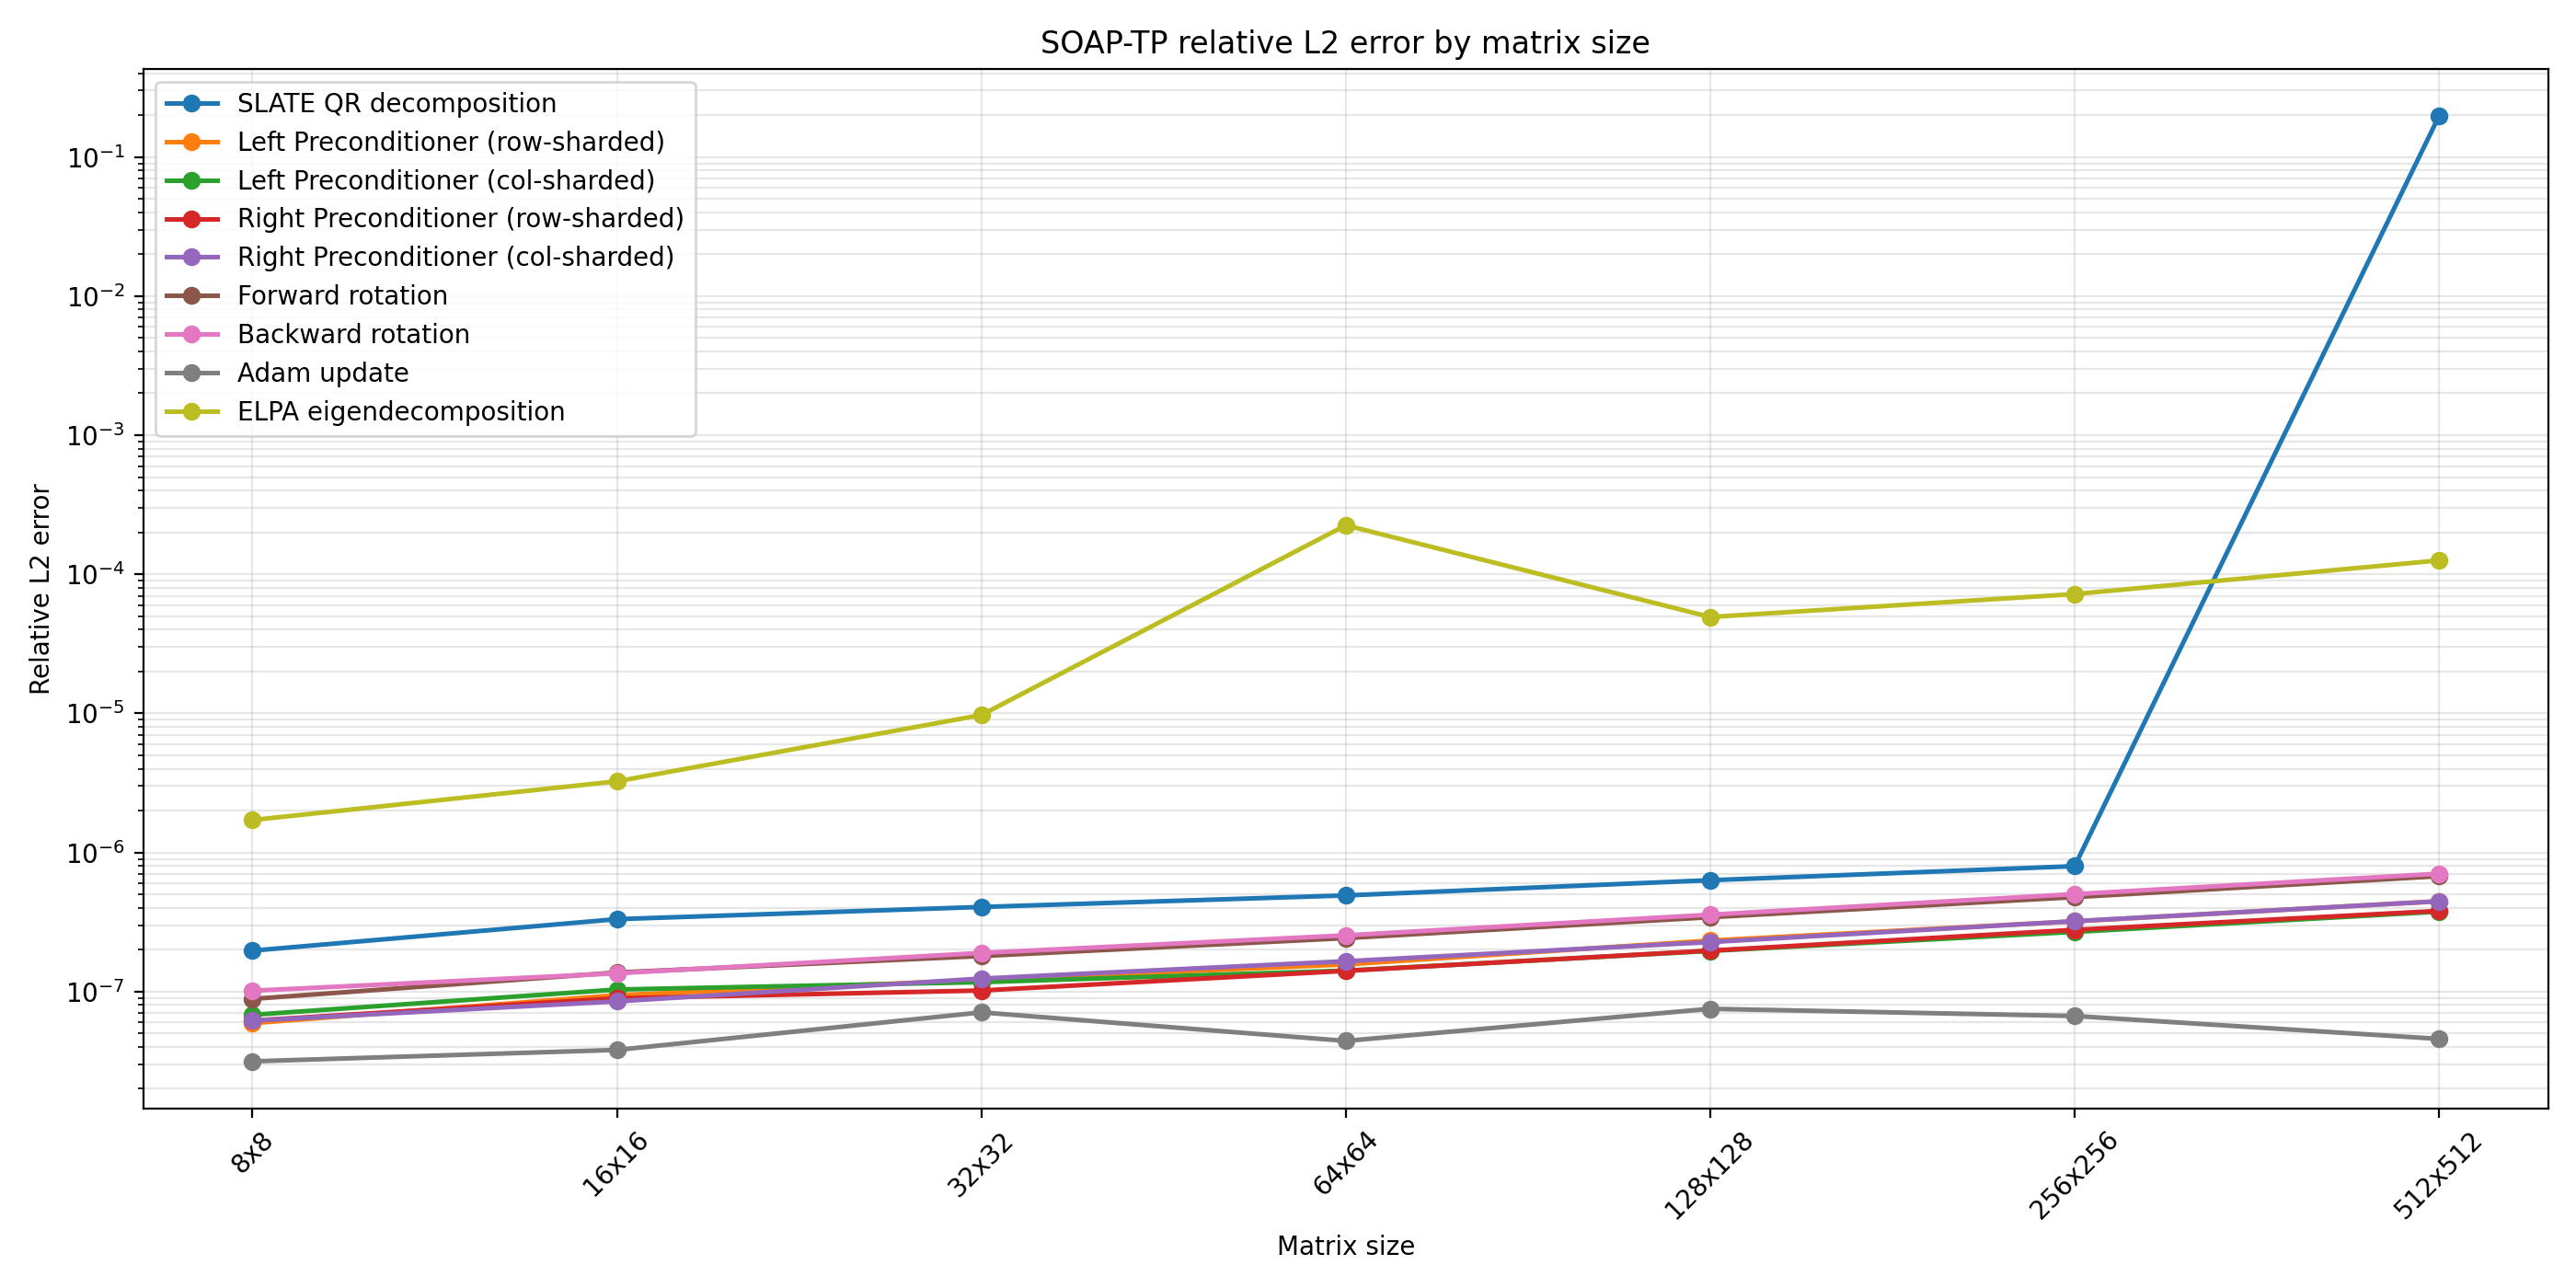
\includegraphics[width=\textwidth]{figures/component_accuracy.png}
    \caption{Relative $L_2$ error of the main SOAP-TP components as matrix size increases. The preconditioner, rotation, and Adam operations remain close to their dense references, while the basis-related operations show greater numerical sensitivity.}
    \label{fig:component-error}
\end{figure}

The four preconditioner paths remain close to the dense reference throughout the tested range. This includes the left and right preconditioners for both row- and column-sharded gradients. Their errors stay around the $10^{-7}$ level through $512\times512$. The forward and backward rotations show similar behavior, while the local Adam update remains below these errors.

The basis operations behave differently. The ELPA eigendecomposition has larger numerical differences than the preconditioner and rotation kernels, reaching approximately the $10^{-4}$ range for some matrix sizes. The SLATE QR result remains relatively close to its reference through $256\times256$, but its error rises sharply at $512\times512$ in this experiment.

This distinction became useful when debugging the complete optimizer. The distributed Gram-matrix construction, rotations, and Adam calculation remained accurate as matrix size increased. The larger deviations were concentrated around the operations used to construct and refresh the SOAP basis.

\subsection{End-to-end SOAP accuracy}

I next compared the final update produced by the distributed SOAP implementation against the reference implementation. Figure~\ref{fig:final-step-accuracy} shows this error across increasing matrix sizes for both row- and column-sharded inputs.

\begin{figure}[htbp]
    \centering
    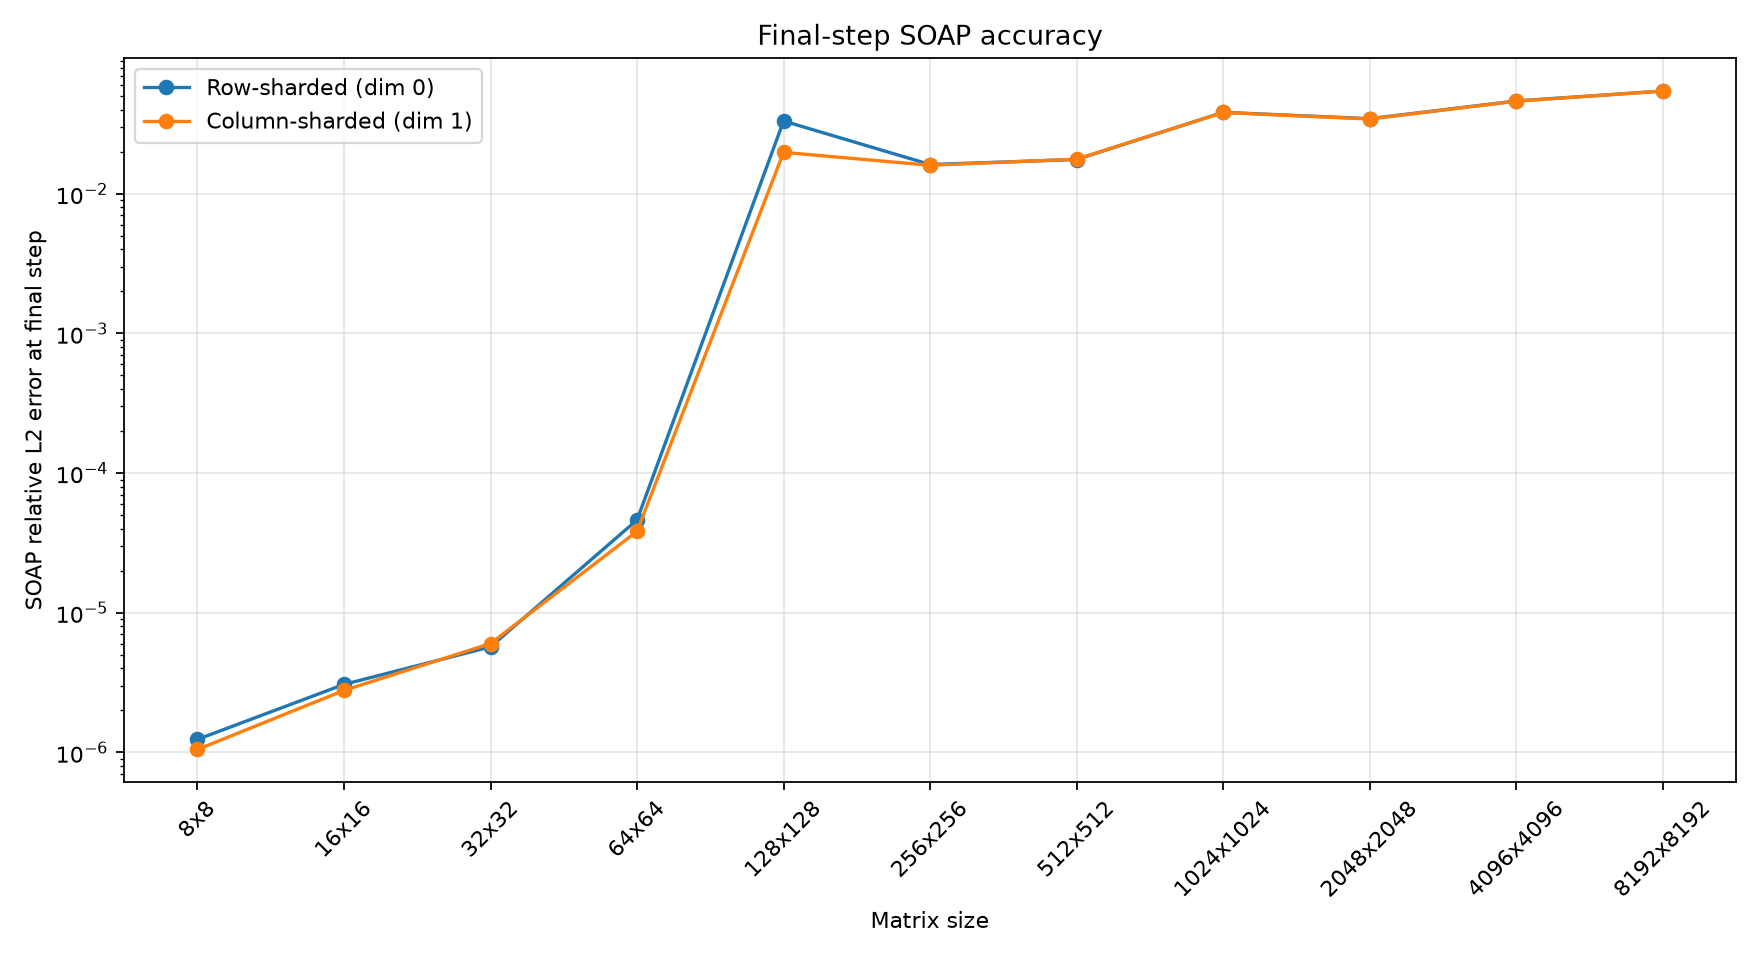
\includegraphics[width=\textwidth]{figures/final_step_accuracy.png}
    \caption{Relative $L_2$ error of the final SOAP update for row- and column-sharded matrices. Both sharding directions show nearly the same trend as matrix size increases.}
    \label{fig:final-step-accuracy}
\end{figure}

For the smaller matrices, the complete distributed update remains very close to the reference. The error is approximately $10^{-6}$ at $8\times8$ and increases gradually through $64\times64$. A much larger change appears at $128\times128$, where the error moves into the percent range.

Beyond this point, the error remains on the order of a few percent and generally increases with matrix size. The largest cases shown in Figure~\ref{fig:final-step-accuracy} approach roughly five percent relative $L_2$ error.

An important feature of the result is how closely the two sharding directions track one another. Row- and column-sharded execution involve different communication patterns when constructing the two preconditioners. Despite this, their final-step errors are almost identical over most of the tested sizes.

This made a sharding-specific implementation error less likely to be the dominant cause of the end-to-end difference. Combined with the component tests, it pointed more strongly toward a part of the algorithm shared by both paths: the SOAP basis.

\subsection{Numerical behavior of the eigenbasis}
\label{sec:numerical-results}

The basis calculation became the main focus of the numerical investigation.

During development, the local reference path used \texttt{torch.linalg.eigh} on a float32 preconditioner. The distributed ELPA path could instead solve the same preconditioner in float64 and cast the resulting basis back to float32.

Changing the arithmetic precision of the eigensolve may appear minor, but the resulting eigenvectors do not have to match elementwise. Their signs can differ, and their ordering can change. Repeated or nearly repeated eigenvalues introduce an additional ambiguity because different orthonormal bases can span the same eigenspace.

SOAP is particularly sensitive to this distinction because the basis defines the coordinates in which Adam operates. The projected gradient is

\begin{equation}
Z_t = Q_L^\top G_t Q_R,
\end{equation}

and the Adam moments are accumulated using entries of $Z_t$. A change in $Q_L$ or $Q_R$ therefore changes the coordinates presented to the elementwise optimizer.

I isolated this effect using a local precision-only experiment. The gradient stream and the rest of the SOAP calculation were kept unchanged while only the precision of the eigendecomposition was changed. The resulting difference in the final SOAP update closely followed the divergence seen between the local and distributed implementations. This indicated that eigensolve precision and the resulting basis choice accounted for a substantial portion of the end-to-end error.

Rank deficiency makes this issue more relevant during initialization. For a matrix gradient,

\begin{equation}
\operatorname{rank}(GG^\top) \leq \min(m,n).
\end{equation}

If $m>n$, the initial left Gram matrix is necessarily rank deficient. The basis within its null space is not unique, so two eigensolvers can return different eigenvectors while still representing the same mathematical subspace.

This also affects how the distributed implementation should be validated. Elementwise eigenvector error can be misleading in the presence of sign changes or degenerate eigenspaces. Eigen residual and orthogonality provide better measures of whether an individual basis is numerically valid. Subspace or projector comparisons are more appropriate when eigenvalues are clustered. For SOAP itself, the final update remains the most useful integrated measure because it captures whether those basis differences actually change the optimizer.

\subsection{Strong scaling}

Finally, I measured the strong-scaling behavior of the complete distributed SOAP path. The matrix size was fixed at $16{,}384\times16{,}384$, while the execution used 1, 2, 4, and 8 GPU ranks. Figure~\ref{fig:strong-scaling} compares the measured speedup with ideal linear scaling.

\begin{figure}[htbp]
    \centering
     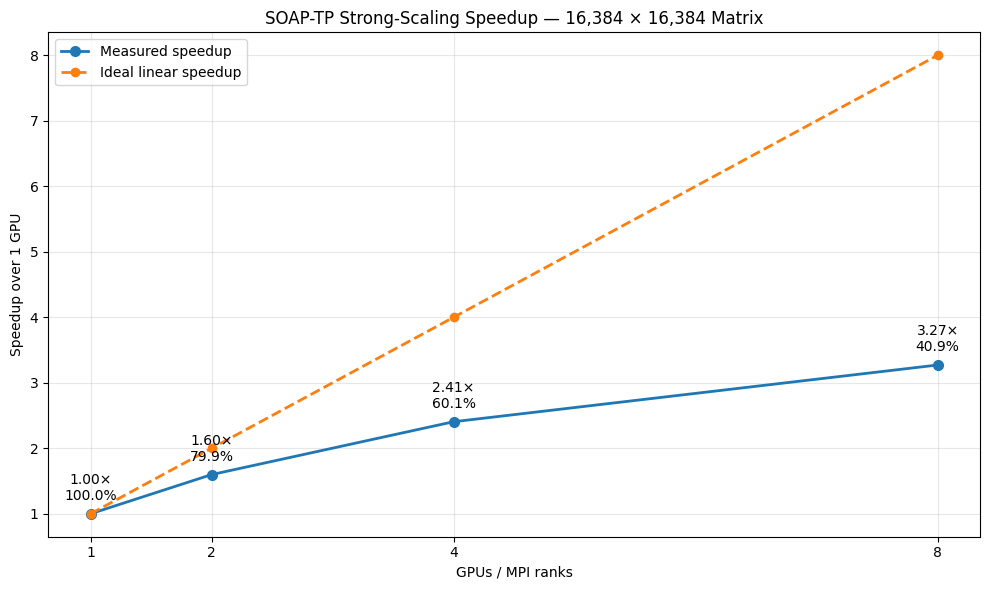
\includegraphics[width=0.9\textwidth]{figures/strong_scaling.png}
    \caption{Strong-scaling speedup for a $16{,}384\times16{,}384$ SOAP-TP workload. The implementation reaches $3.27\times$ speedup on eight GPU ranks, corresponding to approximately 40.9\% parallel efficiency.}
    \label{fig:strong-scaling}
\end{figure}

The average measured SOAP step decreased from approximately 81.9 seconds on one GPU rank to 25.0 seconds on eight ranks. The corresponding eight-GPU speedup is

\begin{equation}
\frac{81.9}{25.0} \approx 3.27.
\end{equation}

The two-GPU run reaches approximately $1.60\times$ speedup, corresponding to 79.9\% parallel efficiency. At four GPUs, the measured speedup is $2.41\times$, or 60.1\% efficiency. Efficiency falls to 40.9\% at eight GPUs.

The implementation therefore benefits from additional GPUs, although the scaling becomes progressively less efficient as the rank count increases. The distributed step includes communication inside the matrix operations as well as synchronization between stages. It also pays for conversion between the tensor-parallel and block-cyclic layouts.

The growing gap from ideal scaling suggests that reducing communication and synchronization will be more important than simply accelerating the local computation. Concurrent execution of the left and right SOAP paths, overlap with backpropagation, and reductions in layout-conversion overhead are therefore natural targets for the next performance pass.

\section{Future Directions}

\subsection{Optimize the current distributed workflow}

The current implementation establishes a working end-to-end path for tensor-parallel SOAP using a two-dimensional block-cyclic representation. The next systems question is how much of its overhead can be removed while preserving the same numerical behavior.

The present workflow contains several distinct distributed stages. Gradients are redistributed from their tensor-parallel layout, the left and right preconditioners are constructed, the bases are computed or refreshed, and the gradient is rotated into and out of the SOAP basis. Each transition introduces some combination of communication, synchronization, or temporary storage.

A useful next step is therefore to profile the complete critical path and optimize the existing design before changing its underlying data model. The left and right preconditioner paths are largely independent until both bases are required for the forward rotation, which creates an opportunity for concurrent execution. There is also room to reduce repeated layout conversion and synchronization between successive matrix operations.

The block size and process-grid configuration should be treated as performance parameters rather than fixed implementation details. Their effect is likely to depend on matrix shape as well as rank count. These experiments would establish how far the current two-dimensional design can be pushed and provide a stronger baseline for more substantial changes to the distribution strategy.

\subsection{Avoid the two-dimensional block-cyclic layout}

The current implementation redistributes tensor-parallel shards into a two-dimensional block-cyclic layout because this representation works naturally with ELPA and SLATE. That redistribution is convenient for dense distributed linear algebra, but it also introduces additional data movement and makes the optimizer maintain a second matrix layout.

A more fundamental question is whether SOAP actually needs this representation.

Tensor-parallel model parameters already have a one-dimensional row- or column-sharded layout. If the required basis operations could be performed directly from that representation, much of the conversion between model and optimizer layouts could disappear.

The main challenge is the eigensolver. Traditional dense distributed eigensolvers are commonly designed around two-dimensional matrix distributions. An alternative path could instead use an iterative distributed basis method that operates over one-dimensional shards. Subspace iteration, Krylov-style methods, or other matrix-vector and matrix-block formulations are possible directions because they can work from distributed matrix products without requiring the complete matrix to be represented in a two-dimensional block-cyclic form.

This raises a broader algorithmic question for SOAP: whether a full dense eigendecomposition is necessary in the first place. If an approximate basis computed directly from the tensor-parallel layout produces equivalent training behavior, the optimizer could use a much simpler distributed representation.

The comparison should therefore include both performance and optimizer accuracy. The existing two-dimensional implementation provides a useful reference for determining how much communication is saved and whether the resulting SOAP update changes materially.

\subsection{Determine whether basis differences matter during training}

The current validation shows that differences in the basis can produce noticeable differences in the final SOAP update. The remaining question is whether those differences have a meaningful effect on training.

A controlled training experiment should vary only the basis path while keeping the model initialization, data order, and optimizer configuration fixed. The local eigensolver, distributed eigensolver, and iterative basis-refresh paths can then be compared through their training trajectories rather than only through individual update tensors.

This experiment would answer an important practical question. SOAP may tolerate basis-level numerical differences even when they appear large in an elementwise comparison. Alternatively, small changes in the basis may accumulate through the Adam moments and eventually alter convergence.

The same experiments can be used to study basis stability across optimizer steps. A useful basis should satisfy the eigenproblem while also avoiding unnecessary changes in the coordinate system seen by the accumulated Adam state. Warm-started basis updates and alignment with the previous basis are natural directions to investigate if temporal instability proves important.

\subsection{Study step directions under rank-deficient preconditioners}

Rank-deficient preconditioners introduce a different question. If a Gram matrix contains repeated zero or nearly zero eigenvalues, its eigenvectors are not uniquely determined within the corresponding subspace. The eigensolver therefore has freedom to return many mathematically valid bases.

For SOAP, that freedom may matter because Adam operates independently along the resulting coordinates. Different choices of basis inside the same degenerate subspace can therefore lead to different optimizer updates.

This suggests a direction beyond simply making the eigensolver more stable: determine whether some valid basis choices produce more useful update directions than others.

One way to study this is to separate the subspace associated with significant eigenvalues from the rank-deficient or nearly degenerate subspace. Within the latter, different orthogonal basis completions can be tested while keeping the represented preconditioner unchanged. Their resulting SOAP updates can then be compared through quantities such as update direction and subsequent loss reduction.

If a consistent relationship exists between the basis choice and the quality of the optimizer step, the arbitrary eigenvector freedom in a rank-deficient preconditioner could become something the optimizer uses deliberately. If no such relationship appears, the simpler objective would be to select the basis that provides the greatest temporal continuity for the Adam state.

\subsection{Overlap SOAP with backpropagation}

The current implementation treats SOAP as a distinct optimizer phase after backpropagation completes. A full training system does not necessarily need to execute the two phases sequentially.

During backpropagation, gradients become available one layer at a time. Once the gradient shard for a layer is complete, some SOAP work for that layer can begin while backpropagation continues through the remaining layers.

The preconditioner update is a natural starting point because it depends only on the completed gradient for that layer. Basis work could follow when a refresh is required. Later stages would continue as their dependencies become available.

The main question is how much of this work can actually be hidden. SOAP and backpropagation compete for GPU compute, memory bandwidth, and communication resources. Running them concurrently is useful only when the overlap reduces the iteration critical path rather than slowing both workloads through contention.

The eventual goal is a pipelined execution model in which the optimizer progresses alongside the backward pass. By the time backpropagation finishes, a substantial fraction of the SOAP work for earlier layers could already be complete. The remaining synchronization would then occur close to the point where the updated parameters are required for the next forward pass.

\bibliographystyle{plainnat}
\bibliography{overleaf/reference}

\end{document}

